\newpage
\section{Parsing}
\begin{itemize}
    \item Lexical Analysis: Create sequence of tokens from characters
    \item Parsing: Create abstract syntax tree from sequence of tokens
\end{itemize}

Syntax: the way in which words are put together to form phrases, clauses, or sentences

\begin{itemize}
    \item Input: sequence of tokens from lexer; 
    \item Output: parse tree of the program (But some parsers never produce a parse tree ...)
\end{itemize}

\begin{figure}[!htb]
    \centering
    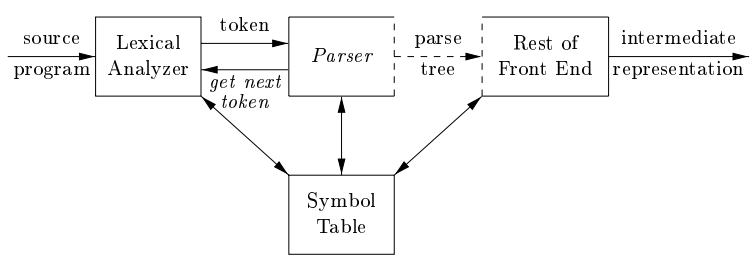
\includegraphics[width=0.42\textwidth]{pic/CP3/compiler.png}
    \caption{compiler}
\end{figure}


\subsection{Context-free Grammars}
\subsubsection{Definition for CFG}
计算理论 IV.1.

\subsubsection{Derivations}
计算理论 IV.2-3

用 CFG 生成 string

\subsubsection{Parse Trees}
计算理论 IV.5

Representing derivations as a tree. Parse trees have meaning. 

\subsubsection{Ambiguous Grammars}
A grammar is ambiguous if the same sequence of tokens can give rise to two or more parse trees.

解决二义性(Ambiguity)的方式就是重写文法. 解决二义性没有通用的方法, 一般都是通过声明 precedence(优先级) 与 associativity(结合性) 来消除文法中的二义性.

\subsubsection{End-Of-File Marker}
Use \$ to represent end of file

\subsection{Predictive Parsing}

\subsubsection{Recursive-Descent Parser}
Each grammar production turns into one clause of a recursive function. 自顶向下分析.

Problem: 预测分析需要每个子表达式的 the first terminal symbol 提供足够的信息来决定生成的是什么.

\begin{definition}[Nullable]
    Non-terminal $X$ is Nullable if $X$ can derive the empty string.
\end{definition}

\begin{definition}[First Sets]
    $First(\gamma)$ is the set of terminals that can begin strings derived from $\gamma$.
    \begin{align*}
        First(X)=\{ t|X\to^*t\alpha \}\cup\{ \epsilon | X\to^*\epsilon \}
    \end{align*}
\end{definition}
即, 如果 $X$ 可以经 0 步或多步推导出以 terminal $t$ 开头的串, 那么 $t$ 属于 ${First}(X)$;如果 $X$ 可以经 0 步或者多步推导出空串, 那么 $\epsilon$ 属于 ${First}(X)$. 

\begin{definition}[Follow Sets]
    $Follow(X)$ is the set of terminals that can immediately follow $X$. That is, $t \in Follow(X)$ if there is any derivation containing $Xt$. This can occur if the derivation contains $XYZt$ where $Y$ and $Z$ both derive $\epsilon$.
    \begin{align*}
        Follow(X)=\{ t|S\to^*\alpha Xt\beta \}
    \end{align*}
\end{definition}

$\epsilon$ 不会出现在 Follow Sets 中. Start Symbol 的 Follow Set 包含文件结束符 \$. 

\begin{algorithm}[H]
    \caption{Compute $First$, $Follow$, and $nullable$}
    \begin{algorithmic}
        \State Initialize $First$ and $Follow$ to all empty sets, and nullable to all false.
        \For{each terminal symbol $t$}
            \State $First(t)\gets \{ t \}$
        \EndFor
        \Repeat
            \For{each production $X\to Y_1Y_2\dots Y_k$}
                \For{each $i$ from $1$ to $k$, each $j$ from $i+1$ to $k$}
                    \If{all the $Y_i$ are nullable}
                        \State $nullable(X)\gets true$
                    \EndIf
                    \If{$Y_1\dots Y_{i-1}$ are all nullable}
                        \State $First(X)\gets First(X)\cup First(Y_i)$
                    \EndIf
                    \If{$Y_{i+1}\dots Y_k$ are all nullable}
                        \State $Follow(Y_i)\gets Follow(Y_i)\cup Follow(X)$
                    \EndIf
                    \If{$Y_{i+1}\dots Y_{j-1}$ are all nullable}
                        \State $Follow(Y_i)\gets Follow(Y_i)\cup First(Y_j)$
                    \EndIf
                \EndFor
            \EndFor
        \Until{$First, Follow$ and nullable didn't change in this iteration.}
    \end{algorithmic}
\end{algorithm}

\subsubsection{Building a Predictive Parser}
\begin{itemize}
    \item $Z\to XYZ | d$
    \item $Y\to c | \epsilon $
    \item $X\to a | Y$
\end{itemize}
\begin{table}[!htb]
    \centering
    \begin{tabular}[c]{cccc}\toprule
        & Nullable & First & Follow \\ \midrule
        $Z$ & no  & $d,a,c$ & \\ \cmidrule{1-1}
        $Y$ & yes & $c$ & $a,c,d $\\ \cmidrule{1-1}
        $X$ & yes & $a,c$ & $a,c,d$\\
        \bottomrule
    \end{tabular}
\end{table}


\subsubsection{Building parsing table}
\begin{itemize}
    \item if $T\in First(s)$ then enter $(X\to s)$ in row $X$, col $T$
    \item if $s$ is Nullable and $T\in Follow(X)$, enter $(X\to s)$ in row $X$, col $T$
\end{itemize}

Build parsing table where row $X$, col $T$ tells parser which clause to execute in function $X$ with next-token $T$:
\begin{table}[!htb]
    \centering
    \begin{tabular}[c]{cccc}\toprule
        & $a$ & $c$ & $d$\\ \midrule
        $Z$ & $Z\to XYZ$ & $Z\to XYZ$ &     \begin{tabular}[c]{@{}l@{}} $Z\to d$ \\ $Z\to XYZ$ \end{tabular} \\ \cmidrule{1-1}
        $Y$ & $Y\to\ $ &     \begin{tabular}[c]{@{}l@{}} $Y\to\ $ \\ $Y\to c$ \end{tabular} & $Y\to\ $ \\ \cmidrule{1-1}
        $X$ &    \begin{tabular}[c]{@{}l@{}} $X\to a$ \\ $X\to Y$ \end{tabular} & $X\to Y$ & $X\to Y$ \\ 
        \bottomrule
    \end{tabular}
\end{table}

\subsubsection{Predictive Parsing: LL(1)}
If a predictive parsing table constructed this way contains no duplicate entries, the grammar is called LL(1).

LL(1): Left-to-right parse, Left-most derivation, 1 symbol lookahead.

In LL(k) parsing table, columns include every k-length sequence of terminals. 

用栈来存储正在生成的 parse tree, 栈顶为 leftmost non-terminal 或即将匹配的 leftmost terminal. 

\begin{example}\quad

    \begin{itemize}
        \item $E\to TX$
        \item $T\to \text{int }Y|(E)$
        \item $X\to +E|\epsilon$
        \item $Y\to *T|\epsilon$
    \end{itemize}
    \begin{table}[!htb]
        \centering
        \begin{tabular}[c]{cccc}\toprule
             & Nullable & First & Follow\\ \midrule
            $E$ & no & $(,\text{int}$ & $),$ \$  \\ \cmidrule{1-1}
            $X$ & yes & $+, \epsilon$ &  $),$ \$ \\ \cmidrule{1-1}
            $T$ & no & $(,\text{int}$ & $+,),$ \$  \\ \cmidrule{1-1}
            $Y$ & yes & $*, \epsilon$ & $+,),$ \$ \\ 
            \bottomrule
        \end{tabular}
    \end{table}

    \begin{table}[!htb]
        \centering
        \begin{tabular}[c]{ccccccc}\toprule
             & int & $*$ & $+$ & $($ & $)$ & \$ \\ \midrule
            $E$ & $TX$ & & $TX$ & & &  \\ \cmidrule{1-1}
            $X$ & & & $+E$ & & $\epsilon$ & $\epsilon$  \\ \cmidrule{1-1}
            $T$ & int $Y$ & & & $(E)$ & &  \\ \cmidrule{1-1}
            $Y$ & & $*T$ & $\epsilon$ & & $\epsilon$ & $\epsilon$  \\ 
            \bottomrule
        \end{tabular}
    \end{table}
    
    \begin{table}[!htb]
        \centering
        % \caption{}
        \begin{tabular}[c]{lll}\toprule
            Stack & Input & Action \\ \midrule
            $E$\$ & $\text{int}*\text{int}$\$ & $TX$\\
            $TX$\$ & $\text{int}*\text{int}$\$ & $\text{int }Y$\\
            $\text{int }YX$\$ & $\text{int}*\text{int}$\$ & terminal\\
            $YX$\$ & $*\text{int}$\$ & $*T$\\
            $*TX$\$ & $*\text{int}$\$ & terminal \\
            $TX$\$ & $\text{int}$\$ & int $Y$ \\
            $\text{int} YX$\$ & $\text{int}$\$ & terminal \\
            $YX$\$ & \$ & $\epsilon$ \\
            $X$\$ & \$ & $\epsilon$ \\
            \$ & \$ & Accept \\
            \bottomrule
        \end{tabular}
    \end{table}
    
\end{example}

\subsubsection{Eliminate left-recursion}
Rewrite the grammar so it parses the same language but the rules are different.

\begin{itemize}
    \item $E\to E+T|T \Rightarrow E\to TE', E'\to +TE'|\epsilon$
    \item $A\to A\alpha | \beta \Rightarrow A\to \beta A', A'\to \alpha A' | \epsilon$
\end{itemize}

\subsubsection{Left Factoring}
提取左因子
\begin{itemize}
    \item $E\to T+E|T \Rightarrow E\to TX, X\to +E|\epsilon$
\end{itemize}

\subsubsection{Error Recovery}
How should error be handled?
\begin{itemize}
    \item Raise an exception and quit parsing
    \item Print an error message and recover from the error
\end{itemize}
This can proceed by deleting, replacing, or inserting tokens

\subsection{LR Parsing}
\subsubsection{Bottom-up Parsing}
自底向上分析.

LL(k) 只看前面 $k$ 个 token.

LR(k): Left-to-right parse, Rightmost derivation, k-token lookahead 可以看到代表输入的全部右侧的生成.

Shift-reduce parsing:
\begin{itemize}
    \item Reduce(规约): token 到 non-terminal
    \item Shift(移进): 右移一位, 考虑下一个 terminal
\end{itemize}

LALR variant: The basis for parsers for most modern programming languages, Implemented in tools such as Yacc.

\begin{figure}[!htb]
    \centering
    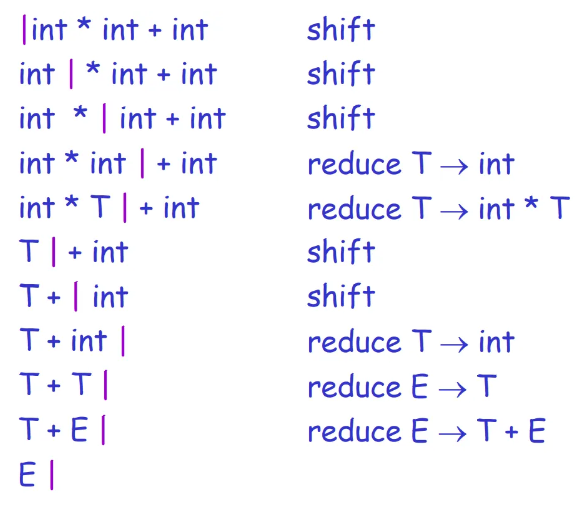
\includegraphics[width=0.309\textwidth]{pic/CP3/lrexp.png}
    \caption{Example}
\end{figure}

\subsubsection{LR Parsing Engine}
The LR parser use a DFA to know when to shift and when to reduce.

Shift-reduce algorithm (details):
\begin{itemize}
    \item The parser summarizes the current ``parse state'' using an integer
    \item Algorithm: Based on next input symbol and the parse state (as opposed to the entire stack), parser table indicates
    \begin{itemize}
        \item $Shift(n)$: Advance input one token; push $n$ on stack.
        \item $Reduce(k)$:
        \subitem Pop stack as many times as the number of symbols on the right-hand side of rule $k$;
        \subitem Let $X$ be the left-hand-side symbol of rule $k$;
        \subitem In the state now on top of stack, look up $X$ to get ``goto $n$''; 
        \subitem Push n on top of stack.
        \item $Accept$: Stop parsing, report success
        \item $Error$: Stop parsing, report failure
    \end{itemize}
\end{itemize}

The elements in the transition table are labeled with four kinds of actions:
\begin{itemize}
    \item $s_n$: Shift into state $n$
    \item $g_n$: Goto state $n$
    \item $r_k$: Reduce by rule $k$
    \item $a$: Accept
    \item $\ $: Error 
\end{itemize}

\begin{example}\quad
    
    \begin{enumerate}
        \item $S\to S;S$
        \item $S\to id:=E$
        \item $S\to print(L)$
        \item $E\to id$
        \item $E\to num$
        \item $E\to E+E$
        \item $E\to (S,E)$
        \item $L\to E$
        \item $L\to L, E$
    \end{enumerate}

    \begin{figure}[!htb]
        \centering
        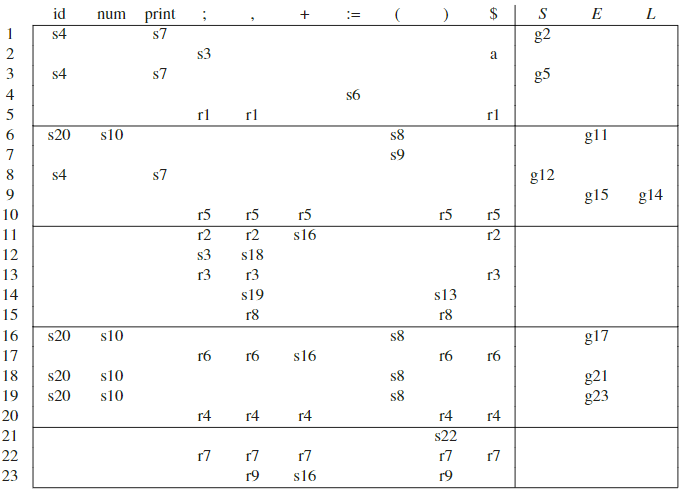
\includegraphics[width=0.42\textwidth]{pic/CP3/lrtable.png}
        \caption{LR parsing table}
    \end{figure}
    
\end{example}

\subsubsection{LR(0) Parsing}
Making shift/reduce decisions without any lookahead.

\begin{figure}[!htb]
    \centering
    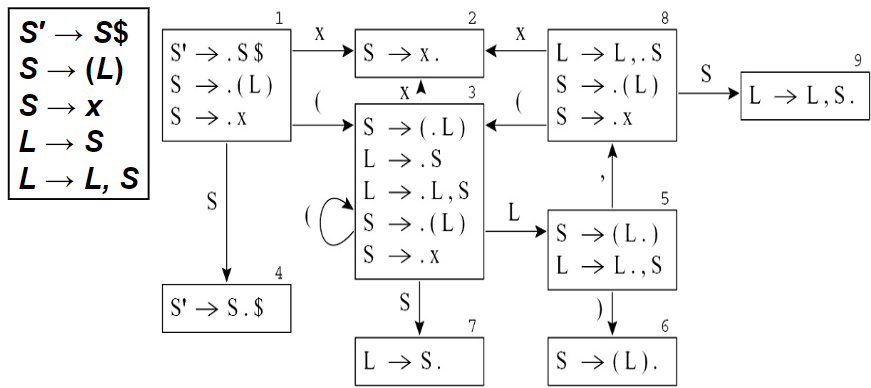
\includegraphics[width=0.42\textwidth]{pic/CP3/LR(0).png}
    \caption{Items and States}
\end{figure}

%TODO 完全听不懂, 回去看辅学()

\subsubsection{SLR Parsing}

\subsubsection{LR(1) Parsing}

\subsubsection{LALR(1) Parsing}

\subsubsection{Hierarchy of Grammar Classes}

\subsubsection{LR Parsing of Ambiguous Grammars}


